%!TEX root = ../thesis.tex

\section{A Metamodel-Independent Syntax}
\label{sec:mmi_syntax}
Section~\ref{subsec:modelling_framework_characteristics} discussed the way in which modelling frameworks implicitly enforce conformance, and hence prevent the loading of non-conformant models. Additionally, modelling frameworks provide little support for checking the conformance of a model with other versions of a metamodel, which is potentially useful during metamodel installation. In Section~\ref{sec:requirements_identification}, these concerns led to the identification of the following requirement: \emph{This thesis must investigate the extension of existing modelling frameworks to support the loading of non-conformant models and conformance checking of models against other metamodels.}

This section describes the way in which existing modelling frameworks load and store models using metamodel-specific binding mechanisms, proposes an alternative binding mechanism using a metamodel-independent syntax, and demonstrates how this facilitates automatic consistency checking. The work presented in this section has been published in \cite{rose09enhanced}.

\begin{figure}[htbp]
	\centering
	\subfigure[Original metamodel.]
	{
	    \label{fig:original_families_mm}
	    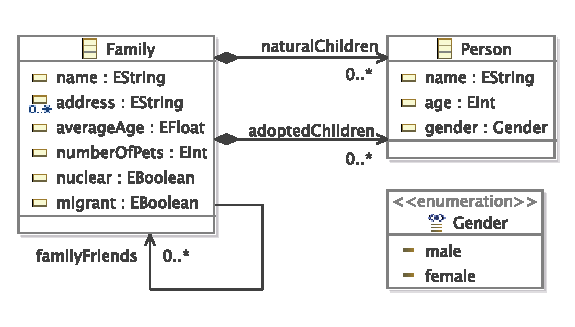
\includegraphics[scale=0.9]{5.Implementation/images/families.pdf}
	}
	\subfigure[Evolved metamodel.]
	{
	    \label{fig:evolved_families_mm}
	    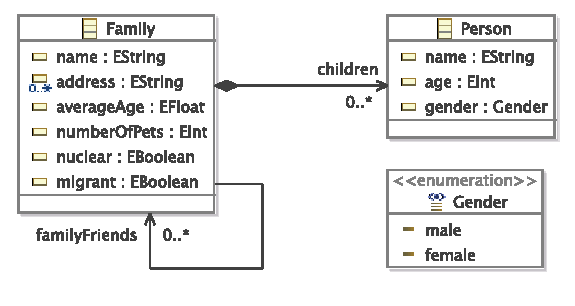
\includegraphics[scale=0.9]{5.Implementation/images/families_evolved.pdf}
	}
	\caption[Evolution of a families metamodel]{Evolution of a families metamodel, based on the metamodel in \cite{hutn}.}
\label{fig:families_mms}
\end{figure}

\subsection{Metamodel Evolution Example: Families}
\label{subsec:families_example}
This section uses the example of metamodel evolution in Figure~\ref{fig:families_mms}. The metamodels in Figure~\ref{fig:families_mms} have been constructed in Ecore, the metamodelling language of EMF, which is based on MOF (Section~\ref{subsec:mof}). The metamodels use Ecore types such as \texttt{ESt\-ri\-ng} and \texttt{EFlo\-at}. The \texttt{nu\-cl\-e\-ar} attribute on the \texttt{Fa\-mi\-ly} type is used to indicate that the family ``comprises only a father, a mother, and children'' \cite{nucleardef}, and not extended family members (such as cousins or grandparents).

In Figure~\ref{fig:original_families_mm}, \texttt{na\-tu\-r\-alCh\-il\-dr\-en} and \texttt{ad\-op\-t\-edCh\-il\-dr\-en} are modelled as separate features, and, in Figure~\ref{fig:evolved_families_mm}, they are modelled as a single feature, \texttt{ch\-il\-dr\-en}. Models that specify values for the \texttt{na\-tu\-r\-alCh\-il\-dr\-en} or \texttt{ad\-op\-t\-edCh\-il\-dr\-en} features do not conform to the evolved metamodel. For example, the model in Figure~\ref{fig:families_model} represents a \texttt{Fa\-mi\-ly} comprising two \texttt{Pe\-rs\-on}s, conforms to the original metamodel, and does not conform to the evolved metamodel. Using the families metamodel and model, the sequel explains why existing modelling frameworks cannot be used to load non-conformant models.

\begin{figure}[htbp]
  \begin{center}
    \leavevmode
    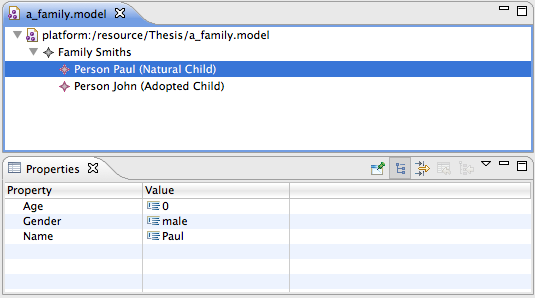
\includegraphics[width=10cm]{5.Implementation/images/family_model.png}
  \end{center}
  \caption[A family model]{A family model, which conforms to the metamodel in Figure~\ref{fig:original_families_mm}, in an EMF tree editor}
  \label{fig:families_model}
\end{figure}


\subsection{Binding to a Specific Metamodel}
\label{subsec:binding_specific}
To load a model, existing modelling frameworks construct objects in the underlying programming language in a process termed \emph{binding} (Section~\ref{subsec:modelling_framework_characteristics}). The metamodel defines the way in which model elements will be bound, and binding is strongly-typed. Figure~\ref{fig:successful_binding} illustrates the results of binding the family model in Figure~\ref{fig:families_model} to the original families metamodel in Figure~\ref{fig:original_families_mm}. The objects in Figure~\ref{fig:successful_binding} instantiate types that are defined in the metamodel, such as \texttt{Fa\-mi\-ly} and \texttt{Pe\-rs\-on}. In other words, binding results in a \emph{metamodel-specific} representation of the model.

\begin{figure}[htbp]
  \centering
  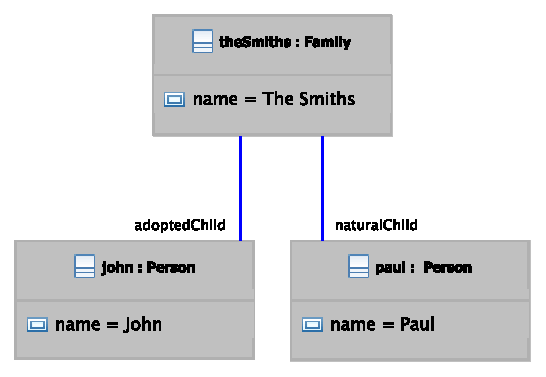
\includegraphics[height=5cm]{5.Implementation/images/successful_binding.pdf}
  \caption[Objects resulting from the binding of a conformant model]{Objects resulting from the binding of a conformant model, as a UML object diagram}
  \label{fig:successful_binding}
\end{figure}

Metamodel-specific binding fails for non-conformant models. For example, attempting to bind the family model in Figure~\ref{fig:families_model} to the evolved families metamodel (Figure~\ref{fig:evolved_families_mm}) fails because the model uses \texttt{na\-tu\-r\-alCh\-il\-dr\-en} and \texttt{ad\-op\-t\-edCh\-il\-dr\-en} features for the type \texttt{Fa\-mi\-ly}, and these features are not defined by the evolved metamodel.

Because non-conformant models cannot be loaded, model migration must be performed by editing the underlying storage representation, which can be error-prone and tedious (Section~\ref{subsec:user-driven_co-evolution}). The sequel discusses potential solutions for loading non-conformant models.

\subsection{Potential Solutions for Loading Non-Conformant Models}
Two potential approaches to binding (and hence loading) non-conformant models have been considered and are now discussed. The benefits and drawbacks of each approach have been compared, which resulted in the selection of the second approach, binding to a metamodel-independent syntax.

\subsubsection{Store metamodel history}
Presently, modelling frameworks are used to store only the latest version of a metamodel, and hence binding fails for models that conform to a previous version of the metamodel. If modelling frameworks could access old versions of a metamodel, models that do not conform to the current version of the metamodel could be loaded by binding to a previous version of the metamodel.

\subsubsection{A metamodel-independent syntax}
Models can always be successfully bound to a \emph{metamodel-independent} representation, such as the one shown in Figure~\ref{fig:minimal_generic_metamodel}. Binding each model element results in the instantiation of a metamodel-independent type (\texttt{Ob\-je\-ct} in Figure~\ref{fig:minimal_generic_metamodel}) rather than of types defined in a specific metamodel, such as \texttt{Fa\-mi\-ly} or \texttt{Pe\-rs\-on}. Hence, binding is independent of the types defined in metamodels, and will succeed for non-conformant models.

\begin{figure}[htbp]
  \centering
  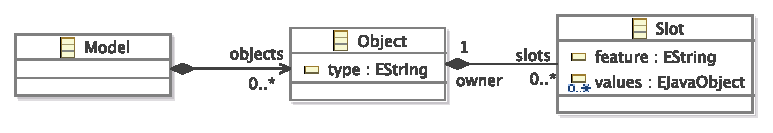
\includegraphics[width=12cm]{5.Implementation/images/slot_model_design.pdf}
  \caption[A minimal generic metamodel for MOF]{A minimal generic metamodel for MOF in Ecore, based on \cite{mof} and taken from \cite{rose09enhanced}.}
  \label{fig:minimal_generic_metamodel}
\end{figure}
   
\subsubsection{Benefits and drawbacks of the potential solutions}
The two potential solutions for loading non-conformant models have different benefits and drawbacks, which are now discussed. Storing metamodel histories would use the binding and conformance checking services provided by existing modelling frameworks, and therefore require less implementation effort than a metamodel-independent syntax, which would require bespoke binding and conformance checking services. Furthermore, structures for managing metamodel histories might be integrated with existing approaches to managing co-evolution, such as metamodel differencing approaches (Sections~\ref{subsec:inference}), for switching between different versions of a MDE workflow.

Storing metamodel histories relies on the metamodel developer to enable model migration: if the metamodel developer does not provide a metamodel that contains historical data, then binding will fail for non-conformant models. Conversely, models can be bound to a metamodel-independent syntax irrespective of the actions of the metamodel developer.

A metamodel-independent syntax has been chosen because it makes fewer assumptions of the metamodel developer, and hence facilitates user-driven as well as developer-driven co-evolution.


\subsection{Proposed Solution: A Metamodel-Independent Syntax}
\label{subsec:binding}
This section discusses the design and implementation of a metamodel-ind\-ep\-en\-de\-nt syntax, and of the binding and conformance checking services that are used to load non-conformant models. As discussed below, the metamodel-independent syntax and conformance checking service are inspired by UML \cite{uml22} and \cite{paige07metamodel}, respectively. As such, the primary contribution of this section is the implementation and integration of the syntax and services with EMF. In addition, the syntax and services have been designed to be re-usable, and hence have been used to simplify the implementation of a textual modelling notation (Section~\ref{sec:notation}) and a model migration language (Section~\ref{sec:flock}).

\subsubsection{Design}
A high-level design for the way in which the metamodel-independent syntax, binding service and conformance checking service load models is shown in Figure~\ref{fig:mmi_workflow}. The \textbf{binding service} parses XMI (the canonical storage representation of models, Section~\ref{subsec:mof}) and produces a model that conforms to the \textbf{metamodel-independent syntax}. The \textbf{conformance checking service} is used to explicitly check the conformance of a model conforming to the metamodel-independent syntax.

\begin{figure}[htbp]
	\centering
		\includegraphics*[viewport=10 590 990 760,width=11.5cm]{5.Implementation/images/mmi_workflow.pdf}
	\caption{Loading models with the metamodel-independent syntax}
	\label{fig:mmi_workflow}
\end{figure}

Binding and conformance checking were split into separate services to facilitate re-use. For example, the textual modelling notation in Section~\ref{sec:notation} re-uses the metamodel-independent syntax and conformance checking service, in conjunction with a different binding service.

\paragraph{Metamodel-independent syntax} The metamodel-independent syntax is used to represent a model without instantiating types defined by its metamodel. Its design was inspired by the metamodel for UML 2 \cite{uml212} object diagrams, which describes objects in a generic, class-independent manner. UML 2 object diagrams are specified in terms of an abstract syntax (comprising, for example, \texttt{InstanceSpecification} and \texttt{Link} classes) and a concrete syntax (comprising, for example, boxes and lines). The metamodel-independent syntax proposed here is abstract. It is not used directly by metamodel developers or users and hence a concrete syntax was not required.

Abstract syntax is typically represented as a metamodel (Section~\ref{subsec:modelling_languages}). The metamodel in Figure~\ref{fig:minimal_generic_metamodel} was used as an initial design for the metamodel-independent syntax, which contains a class for each type in the MOF metamodel that is instantiated in a model. In other words, \texttt{Ob\-je\-ct}s are used to represent each element of a model, and the \texttt{ty\-pe} attribute is used to indicate the name of the metaclass that the \texttt{Ob\-je\-ct} intends to instantiate. Similarly, \texttt{Sl\-ot}s are used to represent values in the model, and the \texttt{feature} attribute indicates the metafeature that the \texttt{Sl\-ot} intends to instantiate. The metamodel was designed to capture the information needed to perform conformance checking (described below), and implementing the conformance checking service led to a refactored metamodel, which is presented in the sequel.

COPE (Section~\ref{subsec:operator-based_co-evolution}) is underpinned by a metamodel-independent syntax. However, the metamodel-independent syntaxes used by COPE and proposed here were developed independently, and both were first published in 2008 (in \cite{rose08hutn,herrmannsdoerfer08cope}).

\paragraph{Metamodel-independent binding service} The metamodel-independent binding service is a text-to-model (T2M) transformation that consumes XMI and produces a model conforming to the metamodel-independent syntax. The transformation was designed to extract all of the information pertaining to the model from XMI, translating it into the concepts defined in the metamodel-independent syntax. In particular, the binding service iterates over each tag in the XMI, and creates instances of \texttt{Ob\-je\-ct} and \texttt{Sl\-ot}. For example, when encountering a tag that represents a model element, the transformation performs the steps in Figure~\ref{fig:binding_objects}.

\begin{figure}[p]
	\begin{framed}
		\begin{enumerate}
			\item Constructs an instance of \texttt{Ob\-je\-ct}, \texttt{o}.
			\item For each attribute of the tag:
			\subitem Creates an instance of \texttt{Sl\-ot}, \texttt{s}.
			\subitem Sets \texttt{s.feature} to the name of the attribute.
			\subitem Sets \texttt{s.value} to the value of the attribute.
			\subitem Adds \texttt{s} to \texttt{o.slots}.
			\item For each child tag:
			\subitem Creates an instance of \texttt{Sl\-ot}, \texttt{s}.
			\subitem Sets \texttt{s.feature} to the name of the child tag.
			\subitem Recursively constructs an instance of \texttt{Ob\-je\-ct}, c.
			\subitem Sets \texttt{s.value} to c.
			\subitem Adds \texttt{s} to \texttt{o.slots}.
		\end{enumerate}
	\end{framed}
	\caption{Pseudo code for binding XMI tags to \texttt{Ob\-je\-ct}s.}
  \label{fig:binding_objects}
\end{figure}

\begin{figure}[p]
  \centering
  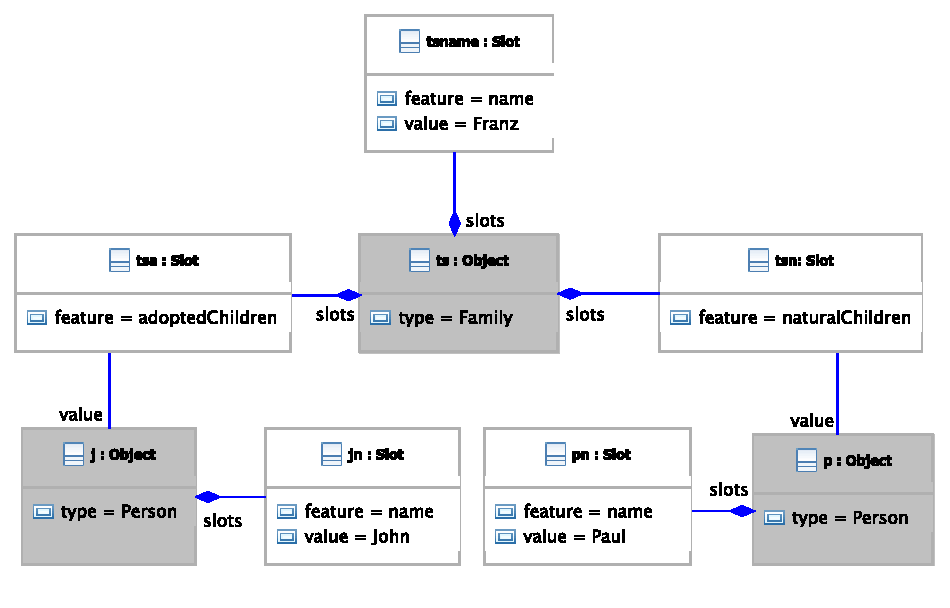
\includegraphics[width=12cm]{5.Implementation/images/generic_binding.pdf}
  \caption[Metamodel-independent binding of the families metamodel]{Result of binding the families model with the metamodel-independent syntax}
  \label{fig:generic_binding}
\end{figure}


Applying the metamodel-independent binding service to the families model (Figure~\ref{fig:families_model}) produces three instances of \texttt{Ob\-je\-ct}, illustrated as a UML object diagram in Figure~\ref{fig:generic_binding}. For clarity, instances of \texttt{Ob\-je\-ct} are shaded, and instances of \texttt{Sl\-ot} are unshaded. The first \texttt{Ob\-je\-ct} represents the \texttt{Fa\-mi\-ly} model element and has three slots. Two of the slots are used to reference the \texttt{Pe\-rs\-on} model elements via the \texttt{na\-tu\-r\-alCh\-il\-dr\-en} and \texttt{ad\-op\-t\-edCh\-il\-dr\-en} references. 


\paragraph{Conformance checking service} Conformance is a type of inter-model consistency, between a model and its metamodel (Section~\ref{subsec:modelling_languages}), and, in MDE, inter-model consistency is often validated using a set of constraints (Section~\ref{subsubsec:model_validation}). Furthermore, \cc conformance can be specified as a set of constraints between a model and its metamodel \cite{paige07metamodel}. As such, the conformance checking service has been designed as the set of constraints between models and metamodels in Figure~\ref{fig:conformance_checking_constraints}.

The conformance checking service must be interoperable with the me\-ta\-mo\-del-ind\-ep\-en\-de\-nt syntax and, hence, the constraints are specified in terms of \texttt{Ob\-je\-ct}s and \texttt{Sl\-ot}s. Clearly, to check conformance the constraints must refer to a (specific) metamodel, and the constraints are also specified in terms of concepts from the MOF metamodelling language (Section~\ref{subsec:mof}), such as \texttt{Class} and \texttt{Property}. Figure~\ref{fig:minimal_mof} shows a minimal version of the MOF metamodel.

\begin{figure}[p]
  \centering
  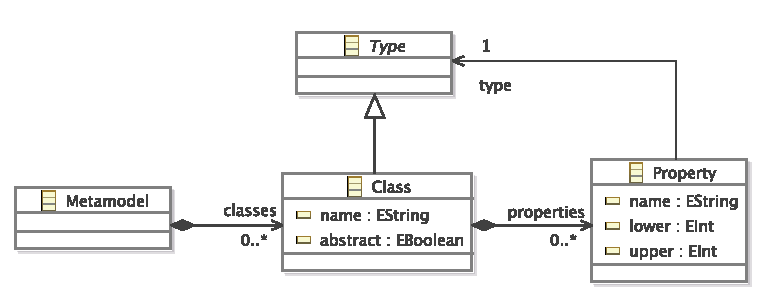
\includegraphics[width=10.5cm]{5.Implementation/images/minimal_mof.pdf}
  \caption{Minimal MOF metamodel, based on \cite{mof}.}
  \label{fig:minimal_mof}
\end{figure}

\begin{figure}[p]
	\begin{framed}
	  \begin{enumerate}
			\item Each \texttt{Ob\-je\-ct}'s \texttt{ty\-pe} must be the \texttt{na\-me} of some non-\texttt{ab\-str\-act} metamodel \texttt{Cl\-a\-ss}.
			\item Each \texttt{Ob\-je\-ct} must specify a \texttt{Sl\-ot} for each mandatory \texttt{Pr\-op\-er\-ty} of its \texttt{ty\-pe}.
			\item Each \texttt{Sl\-ot}'s \texttt{fe\-at\-u\-re} must be the name of a metamodel \texttt{Pr\-op\-er\-ty}. That \texttt{Pr\-op\-er\-ty} must belong to the \texttt{Sl\-ot}'s \texttt{ow\-n\-er}'s \texttt{ty\-pe}.
			\item Each \texttt{Sl\-ot} must be multiplicity-compatible with its \texttt{Pr\-op\-er\-ty}. More specifically, each \texttt{Sl\-ot} must contain at least as many values as its \texttt{Pr\-op\-er\-ty}'s \texttt{lo\-w\-er} bound, and at most as many values as its \texttt{Pr\-op\-er\-ty}'s \texttt{up\-p\-er} bound.
		  \item Each \texttt{Sl\-ot} must be type-compatible with its \texttt{Pr\-op\-er\-ty}. (The way in which type-compatibility is checked depends on the way in which the modelling framework is implemented).
		\end{enumerate}
	\end{framed}
  \caption{The constraints of the conformance checking service.}
  \label{fig:conformance_checking_constraints}
\end{figure}

After binding to the metamodel-independent syntax, the conformance of a model can be checked against any specific metamodel. To illustrate the value of the conformance checking service, consider again the metamodel evolution in Figure~\ref{fig:families_mms} and the bound model in Figure~\ref{fig:generic_binding}. For the evolved metamodel (Figure~\ref{fig:evolved_families_mm}), conformance checking for the model element representing the \texttt{Fa\-mi\-ly} would fail. As illustrated in Figure~\ref{fig:generic_binding}, the \texttt{Fa\-mi\-ly} \texttt{Ob\-je\-ct} defines slots for features named  \texttt{na\-tu\-r\-alCh\-il\-dr\-en} and \texttt{ad\-op\-t\-edCh\-il\-dr\-en}, which are not defined the metaclass \texttt{Fa\-mi\-ly} in Figure~\ref{fig:evolved_families_mm}. Specifically, the model element representing the \texttt{Fa\-mi\-ly} does not satisfy conformance constraint 3, which states: \emph{each \texttt{Sl\-ot}'s \texttt{fe\-at\-u\-re} must be the name of a metamodel \texttt{Pr\-op\-er\-ty}. That \texttt{Pr\-op\-er\-ty} must belong to the \texttt{Sl\-ot}'s \texttt{ow\-n\-er}'s \texttt{ty\-pe}}. The conformance checking service provides a report of conformance problems, which can be used during co-evolution by tools and users.

\subsubsection{Reference implementation in Java, EMF and Epsilon}
\label{subsubsec:mmi_impl}
Reference implementations of the metamodel-independent syntax, the binding service and the conformance service were constructed with Java, EMF and Epsilon (Section~\ref{sec:mde_tools}). The way in which each component was implemented is now discussed.

\paragraph{Metamodel-independent syntax} Ecore, the metamodelling language of EMF, was used to implement the metamodel-independent syntax. The final metamodel is shown in Figure~\ref{fig:mmi_syntax_impl}, which differs slightly from the initial design (Figure~\ref{fig:minimal_generic_metamodel}). Specifically, \texttt{Sl\-ot} is abstract, has a generic type (\texttt{T}), and is the superclass of \texttt{Att\-ri\-bu\-teSl\-ot}, \texttt{Re\-fe\-re\-n\-ceSl\-ot} and \texttt{Co\-nt\-ai\-nm\-entSl\-ot}. These changes simplified the implementation of the (abstract) \texttt{ty\-peCo\-mp\-at\-ib\-i\-leWi\-th} method, which is used by the conformance checking service, and returns \texttt{true} if and only if every element of the \texttt{va\-lu\-es} attribute is type compatible with the \texttt{EC\-la\-ss\-if\-ier} parameter (a metamodel type).  

\begin{figure}[htbp]
  \centering
  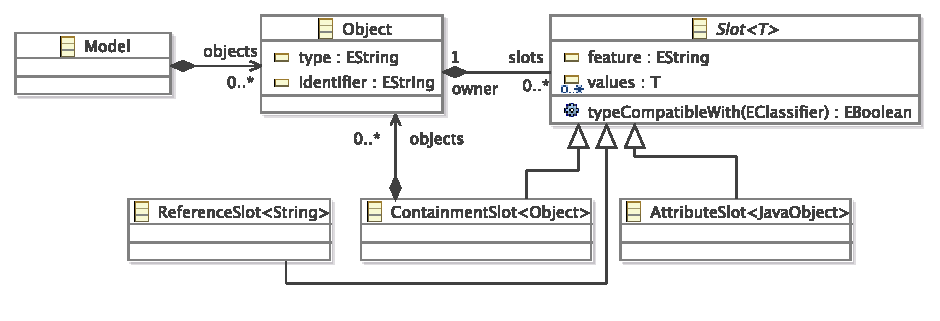
\includegraphics[width=12cm]{5.Implementation/images/slot_model_complete.pdf}
  \caption[Implemented version of the metamodel-independent syntax]{Implemented version of the metamodel-independent syntax, in Ecore}
  \label{fig:mmi_syntax_impl}
\end{figure}

\paragraph{Binding service} A text-to-model (T2M) transformation language (Section~\ref{subsubsec:model_transformation}) could have been used to implement the binding service. However, when this work started (2008) the Eclipse Modeling Project\footnote{\url{http://www.eclipse.org/modeling/}} did not provide a standard T2M language and using a T2M language that was not part of the Eclipse Modeling Project would have complicated installation of the service for users.

Instead, the binding service has been implemented by constructing in Java an XMI parser that emits objects conforming to the metamodel-independent syntax. Listing~\ref{lst:xmi_parser} illustrates the way in which XMI attributes are parsed. The \texttt{pr\-oc\-e\-ssAtt\-rib\-ut\-es} method is called to generate instances of \texttt{At\-tr\-ibu\-teSl\-ot} from the metamodel-independent syntax (Figure~\ref{fig:mmi_syntax_impl}). For each attribute in an XMI tag, the body of the loop is executed. If the attribute is not XMI metadata such as type information (line 4), the name and value of the attribute (lines 5 and 6) are extracted from the XMI, and used to add the value to an \texttt{At\-tr\-ibu\-teSl\-ot} with feature equal to the name of the attribute (line 8). Constructing \texttt{O\-bj\-e\-ct}s and \texttt{Sl\-ot}s is the responsibility of the \texttt{ge\-ne\-ra\-tor} object, which is an instance variable of the parser.


\begin{lstlisting}[caption=Parsing XMI attributes (in Java), label=lst:xmi_parser, language=Java]
private void processAttributes(Attributes atts) {
	for (int index = 0; index < atts.getLength(); index++) {
		
		if (!attributeIsMetadata(atts.getQName(index))) {
			final String feature = atts.getLocalName(index);
			final String value   = atts.getValue(index);
			
			generator.addAttributeValue(feature, value);
		}
	}
}
\end{lstlisting}

\paragraph{Conformance checking service} EVL (Section~\ref{subsubsec:model_validation}), a language tailored for model verification and hence suitable for rapid prototyping of consistency constraints, was used to implement the conformance constraints (Figure~\ref{fig:conformance_checking_constraints}). Listing~\ref{lst:conformance_constraint} shows the EVL constraint that checks whether each \texttt{Ob\-je\-ct}'s \texttt{ty\-pe} is a non-abstract class (constraint 1 in Figure~\ref{fig:conformance_checking_constraints}). The \texttt{ch\-e\-ck} part (line 3) verifies that a particular \texttt{Ob\-je\-ct} (referenced via the \texttt{se\-lf} keyword) refers to a metamodel type that is not abstract. If the check fails, the message (line 4) is automatically added to a set of unsatisfied constraints. The \texttt{toCl\-a\-ss} operation (lines 8-10) is used to determine the metamodel class (an instance of \texttt{EClass}) to which the \texttt{type} attribute (a \texttt{St\-ri\-ng}) of an \texttt{Ob\-je\-ct} refers. The conformance checking service returns a report of unsatisfied constraints.

Type-compatibility checks have been implemented using the type-checking methods provided by EMF. The EVL constraints call the \texttt{isTy\-peCo\-mp\-at\-ib\-leWi\-th} method on the \texttt{Sl\-ot} class. Each subclass of \texttt{Sl\-ot} provides an implementation of \texttt{isTy\-peCo\-mp\-at\-ib\-leWi\-th}, which delegates to EMF to perform type-checking.

\begin{lstlisting}[caption={[Consistency constraint for instantiating a metamodel type]A constraint (in EVL) to check that only concrete metamodel types are instantiated}, label=lst:conformance_constraint, language=EVL, float=tb]
context Object {
	constraint ClassMustNotBeAbstract {
		check: not self.toClass().isAbstract()
		message: 'Cannot instantiate the abstract class: ' + self.type
	}
}

operation Object toClass() : EClass {
	return Metamodel!EClass.all.selectOne(c|c.name == self.type);
}
\end{lstlisting}

% Conformance constraints vary over modelling languages. For example, Ecore, the modelling language of EMF, is similar to but not the same as MOF. Metamodel features defined in Ecore can be marked as transient (not stored to disk) or unchangeable (read-only). Consequently in EMF, conformance constraints are required to restrict the feature value of slots to only non-transient, changeable features.

\subsection{Applications of the Metamodel-Independent Syntax} 
There \changed{``Structures built atop'' changed to ``Applications of''} are many potential uses for the metamodel-independent syntax described in this section. Section~\ref{sec:notation} describes a textual modelling notation integrated with the metamodel-independent syntax to achieve live conformance checking. In addition to this, the metamodel-independent syntax is potentially useful during metamodel installation. As discussed in Section~\ref{subsec:modelling_framework_characteristics}, metamodel developers do not have access to downstream models, and conformance is implicitly enforced by modelling frameworks. Consequently, the conformance of models may be affected by the installation of a new version of a metamodel, and the conformance of models cannot be checked during installation. Typically, installing a new version of a metamodel can result in models that no longer conform to their metamodel and cannot be used with the modelling framework. Moreover, a user discovers conformance problems only when attempting to use a model after installation has completed, and not as part of the installation process.

To \cc enable conformance checking during metamodel installation in EMF, the me\-ta\-mo\-del-ind\-ep\-en\-de\-nt syntax has been integrated with a model indexing service, Concordance \cite{rose10concordance}. The work was conducted outside of the scope of the thesis, and is now summarised to indicate the usefulness of the metamodel-independent syntax for supporting the automation of co-evolution activities. Concordance provides a mechanism for resolving inter-model references (such as those between models and their metamodels). Without Concordance, determining the the instances of a metamodel is possible only by checking every model in the workspace. Integrating Concordance and the metamodel-independent syntax resulted in a service, which Epsilon (Section~\ref{subsec:epsilon}) executes after the installation of a metamodel, to identify the models that are affected by the metamodel changes. All models that conform to the old version of the metamodel are checked for conformance with the new metamodel. As such, conformance checking occurs automatically and immediately after metamodel installation. Conformance problems are detected and reported immediately, rather than when an affected model is next used. Conformance problems detected via Concordance can be reconciled with the structures described in Sections~\ref{sec:notation} and~\ref{sec:flock}.

\subsubsection{Summary}
Modelling frameworks implicitly enforce conformance, which presents challenges for managing co-evolution. In particular, detecting and reconciling conformance problems involves managing non-conformant models, which cannot be loaded by modelling frameworks and hence cannot be used with model editors or model management operations. The metamodel-independent syntax proposed in this section enables modelling frameworks to load non-conformant models, and has has been integrated with Concordance \cite{rose10concordance} to facilitate the reporting of conformance problems during metamodel installation. The metamodel-independent syntax, binding service and conformance checking service underpin the implementation of the textual modelling notation presented in the sequel. The benefits and drawbacks of the metamodel-independent syntax in the context of user-driven co-evolution are explored in Chapter~\ref{Evaluation}. 
